\documentclass[a4paper, 12pt]{article}
\usepackage[T2A]{fontenc}
\usepackage[utf8]{inputenc}
\usepackage[english,russian]{babel}
\usepackage{amsmath, amsfonts, amssymb, amsthm, mathtools, misccorr, indentfirst, multirow}
\usepackage{wrapfig}
\usepackage{graphicx}
\usepackage{subfig}
\usepackage{enumitem}
\usepackage{adjustbox}
\usepackage{pgfplots}
\usepackage{caption}

\usepackage{geometry}
\geometry{top=20mm}
\geometry{bottom=20mm}
\geometry{left=20mm}
\geometry{right=20mm}
\newcommand{\angstrom}{\textup{\AA}}
\begin{document}
	\begin{titlepage}
		\begin{center}
		МИНИСТЕРСТВО ОБРАЗОВАНИЯ И НАУКИ РОССИЙСКОЙ ФЕДЕРАЦИИ\\
		\footnotesize{Московский физико-технический институт}\\
		\footnotesize{(государственный университет)}\\
		\vfill
		{\LARGE
		\textbf{Определение ширины запрещенной зоны полупроводников по спектральной зависимости собственной фотопроводимости}\\
		}
		\vspace{1cm}
		Лабораторная работа по курсу\\
		тведотельная электроника
		\vfill
		\begin{flushright}
			Выполнили: студенты 654 группы.\\
			Нехаев А.С.\\
		\end{flushright}
		\vfill
		г. Долгопрудный\\
		\the\year\:год
		\end{center}
	\end{titlepage}
	\newpage
	\pagenumbering{arabic}
	\tableofcontents
	\newpage
	\section{Цели и задачи исследования}
	\begin{enumerate}
		\item Ознакомление с основами теории собственной фотопроводимости полупроводников;
		\item Определение ширины запрещённой зоны кремния по спектральной зависимости собственной фотопроводимости;
		\item Определение скорости поверхностной рекомбинации.
    \end{enumerate}
    \section{Теоретическая часть}
    При воздействии на полупроводник излучения с энергией кванта $h\nu$, превышающей ширину запрещённой зоны $E_g$ в зоне проводимости, и соотвественно в валентной зоне возникают неравновесные электроны и дырки. Их появление связано с переходами электронов из валентной зоны проводимости. В результате увеличивается проводимость кристалла. Это явление называется собственной фотопроводимостью.

    В непрямозонных полупроводниках типа германия и кремния минимум зоны проводимости и максимум валентной зоны расположены в различных точках зоны Бриллюэна. В этом случае оптический переход электрона из вершины валентной зоны в минимум зоны проводимости возможен лишь при участии третьей частицы – фонона. В соответствии с законом сохранения импульса квазиимпульс такого фонона $q_{\text{ф}}\approx\hbar k_{\text{Б}}$, а энергия $\hbar\omega$ должна удовлетворять закону сохранения энергии:
    \begin{equation}
        h\nu = E_g\pm \hbar\omega_q+\hbar^2(k_n-k_c)^2/2m_n+\hbar^2k_p^2/2m_p
    \end{equation}
    где $k_n$ и $k_p$ -- начальные волновые числа электрона и дырки, а $k_c$ -- конечное волновое число электрона.

    Таким образом, край основной полосы поглощения в полупроводниках типа кремния и германия определяется непрямыми оптическими переходами, сопровождающимися поглощением и испусканием фононов. При этом для разрешённых переходов, которые доминируют в полупроводниках такого типа, коэффициент поглощения:

    \begin{equation}
        K=C\left[\frac{(h\nu-E_g+\hbar\omega_q)^2}{\exp{\frac{\hbar\omega_q}{kT}}-1}+\frac{(h\nu-E_g-\hbar\omega_q)^2}{1-\exp{-\frac{\hbar\omega_q}{kT}}}\right]
    \end{equation}
    При больших энергиях квантов $h\nu>(E_g+\hbar\omega_q)$ начинают преобладать переходы с эмиссией фононов и зависимость $K^{1/2}$ от $h\nu$ должна аппроксимироваться прямой, пересекающей ось энергии в точке $h\nu_1=E_g+\hbar\omega_q$.

    При рассмотрении случая сильного поглощения излечения в образце (оптически толстый образец), то есть при $d/K<<1$, где $d$ -- толщина образца, скорость генерации электронно-дырочных пар экспоненциально уменьшается от поверхности вглубь образца:
    \begin{equation}
        g(x)\approx K(1-R)N_0\exp{-Kx}
    \end{equation}
    где $R$ -- коэффициент отражения света, а $N_0$ -- поток квантов на единицу поверхности.

    Неоднородная германия электронов и дырок в направлении освещения приводит к появлению диффузионно-дрейфовых потоков носителей заряда: быстро диффундирующие носители (электроны) опережают медленные (дырки), что приводит к возникновению электрического поля, ускоряющего медленные носители и замедляющего быстрые и к появлению дрейфовых составляющих потоков. При этом изменение проводимости $\Delta\Sigma$ существенным образом зависит от граничных условий на поверхности образца:
    \begin{equation}
        \Delta\Sigma\sim N_0\left(1+\frac{S}{D}\frac{1}{K}\right)
    \end{equation}
    где $S$ -- скорость поверхностной рекомбинации, $D$ -- коэффициент амбиполярной диффузии.
    
    \section{Экспериментальная часть}
    Для изменения фотоответа полупроводника $\Delta\Sigma$ образец включается последовательно с нагрузочным сопротивлением и источником постоянного напряжения. При освещении проводимость образца возрастает, происходит перераспределение напряжение между образцом и нагрузкой. В результате падение напряжения $U$ на образце при малом относительном увеличении проводимости уменьшается на величину
    \begin{equation}
        \Delta U=\varepsilon\frac{R_H\cdot R_0^2}{(R_H+R_0)^2}\Delta\Sigma
        \label{eq:deltaU}
    \end{equation}
    где $\varepsilon$ -- постоянное напряжение, $R_H$ и $R_0$ -- сопротивление нагрузки и образца, $\Sigma$ -- проводимость.

    Для повышения чувствительности измерения обычно проводят при периодическом прерывании светового потока. При этом соотношение (\ref{eq:deltaU}) характеризует амплитуду отрицательных импульсов напряжения на концах образца. Для исследования интересующих нас зависимостей $\Delta\Sigma/N_0$ от энергии кванта $h\nu$ наряду с $\Delta U$ необходимо знать спектральное распределение интенсивности источника излучения $N_0(h\nu)$.
    \begin{figure}[!htb]
        \centering
        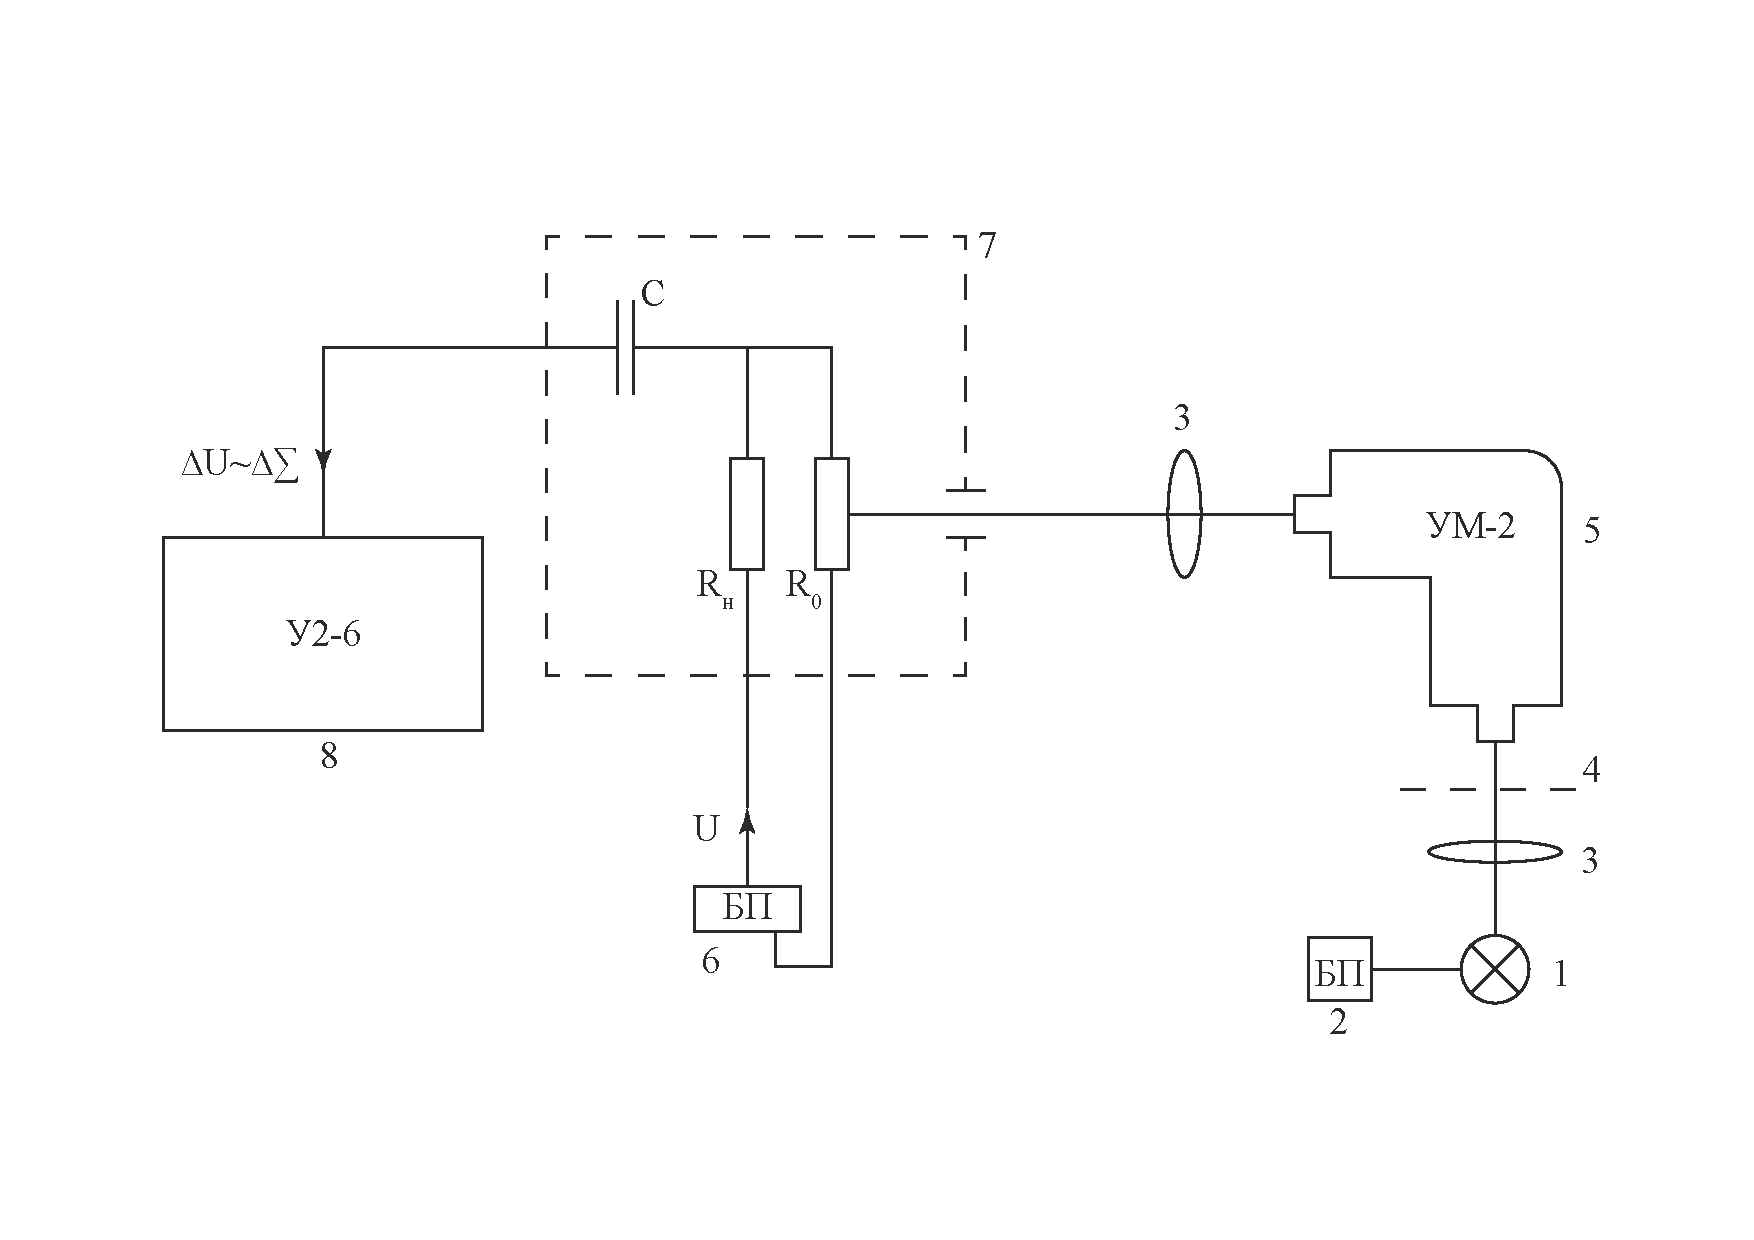
\includegraphics[width=\textwidth]{exp_scheme.pdf}
        \caption{Схема экспериментальной установки. 1 -- осветитель, 2 -- блок питания осветителя, 3 -- линзы, 4 -- механический модулятор излучения, 5 -- монохроматор, 6 -- блок питания образца, 7 -- схема включения образца, 8 -- усилитель}
    \end{figure}
    \section{Ход работы}
    \subsection{Кремний}
    Включаем лампу накаливания и фокусируем излучение монохроматора на образец Si. Подаём постоянное смещение $U$ на образец от источника напряжения. Вращая барабан длин волн, снимаем зависимость сигнала фотопроводимости $\Delta U$ от длины волны излучения. С помощью графика спектрального распределения интенсивности лампы составляем таблицу $\Delta U/I_0$ от делений барабана. С помощью градуировочной кривой переводим деления барабана в энергии кванта $h\nu$. Получаем зависимость $h\nu\Delta U/I_0$, после чего строим зависимость $\sqrt{h\nu\Delta U}/I_0$.
    \begin{figure}[!htb]
        \centering
        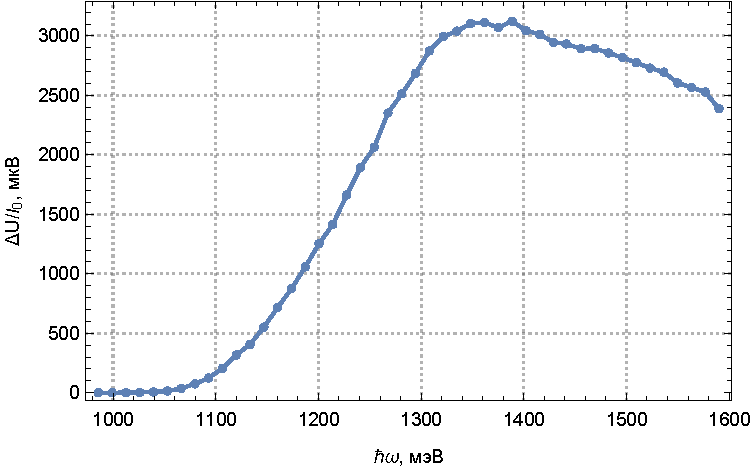
\includegraphics[scale=1]{plot1.pdf}
        \caption{Зависимость $h\nu\Delta U/I_0$ от $\hbar\omega$ для Si.}
    \end{figure}
    \begin{figure}[!htb]
        \centering
        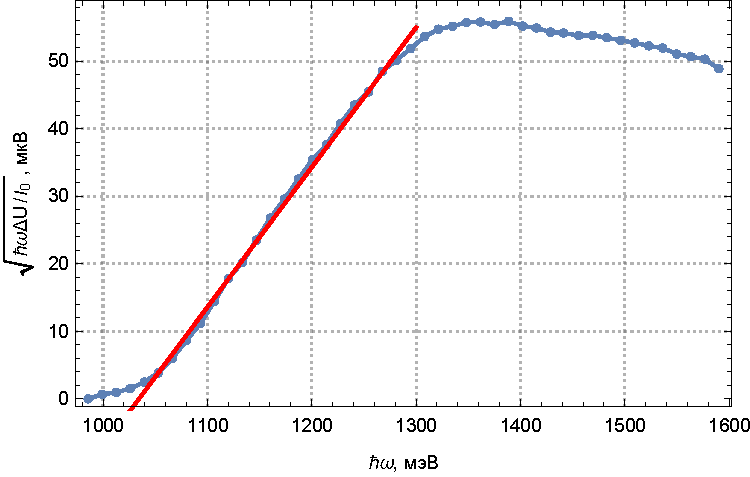
\includegraphics[scale=1]{plot2.pdf}
        \caption{Зависимость $\sqrt{h\nu\Delta U}/I_0$ от $\hbar\omega$ для Si.}
    \end{figure}
    \begin{table}[!htb]
        \caption{Параметры аппроксимации}
        \centering
        \begin{tabular}{l|llll}
        \text{} & \text{Estimate} & \text{Standard Error} & \text{t-Statistic} & \text{P-Value} \\
       \hline
        1 & -214.171 & 3.83204 & -55.8897 & \text{7.99$\cdot 10^{-19}$} \\
        x & 0.207038 & 0.00322285 & 64.2407 & \text{9.98$\cdot 10^{-20}$} \\
    \end{tabular}    
    \end{table}

    Аппроксимируя линейный участок графика до оси энергии, получаем величину $E_g+\hbar\omega_{ph}$ как точку пересечения прямой с осью. Учитывая энергию фонона $\hbar\omega_{ph}=50$ мэВ, находим ширину запрещённой зоны кремния $E_g=1084.45$ мэВ.
    
    \subsection{Селенид кадмия}
    Схожую операцию проделываем для образца CdSe. Получаем зависимость $h\nu \Delta U/I_0$, после чего строим график зависимости $(h\nu\Delta U)^2/I_0$.
    \begin{figure}[!htb]
        \centering
        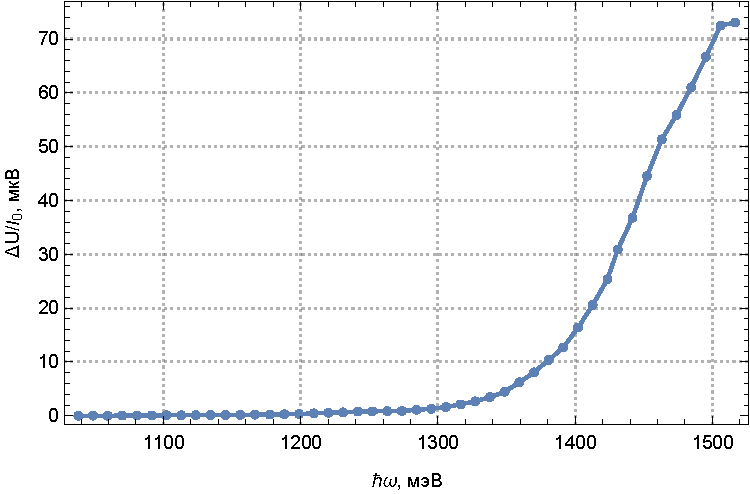
\includegraphics[scale=0.92]{plot3.pdf}
        \caption{Зависимость $h\nu\Delta U/I_0$ от $\hbar\omega$ для CdSe.}
    \end{figure}
    \begin{figure}[!htb]
        \centering
        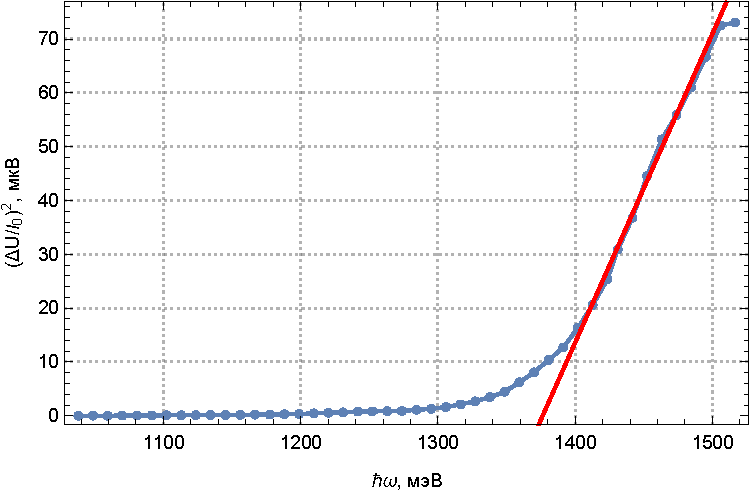
\includegraphics[scale=0.95]{plot4.pdf}
        \caption{Зависимость $(h\nu\Delta U)^2/I_0$ от $\hbar\omega$ для CdSe.}
    \end{figure}
    \begin{table}[!htb]
        \centering
        \caption{Параметры аппроксимации}
        \begin{tabular}{l|llll}
            \text{} & \text{Estimate} & \text{Standard Error} & \text{t-Statistic} & \text{P-Value} \\
           \hline
            1 & -789.897 & 37.1082 & -21.2863 & 0.0000287995 \\
            x & 0.57392 & 0.0254531 & 22.5481 & 0.0000229106 \\
        \end{tabular}
    \end{table}

    Аппроксимируя линейный участок графика до оси энергии, получаем величину $E_g+\hbar\omega_{ph}$ как точку пересечения прямой с осью. Учитывая энергию фонона $\hbar\omega_{ph}=50$ мэВ, находим ширину запрещённой зоны кремния $E_g=1426.32$ мэВ.
    \section{Выводы}
    \begin{enumerate}
        \item Изучили принципы собственной фотопроводимости в полупроводниках
        \item При проведении работы нашли ширину запрещённой зоны кремния и селенида кадмия: 1084.45 мэВ и 1426.32 мэВ соотвественно.
    \end{enumerate}
    \end{document}
